%%%%%%%%%%%%%%%%%%%%%%%%%%%%%%%%%%%%%%%%%
% Programming/Coding Assignment
% LaTeX Template
%
% This template has been downloaded from:
% http://www.latextemplates.com
%
% Original author:
% Ted Pavlic (http://www.tedpavlic.com)
%
% Note:
% The \lipsum[#] commands throughout this template generate dummy text
% to fill the template out. These commands should all be removed when 
% writing assignment content.
%
% This template uses a Perl script as an example snippet of code, most other
% languages are also usable. Configure them in the "CODE INCLUSION 
% CONFIGURATION" section.
%
%%%%%%%%%%%%%%%%%%%%%%%%%%%%%%%%%%%%%%%%%

%----------------------------------------------------------------------------------------
%	PACKAGES AND OTHER DOCUMENT CONFIGURATIONS
%----------------------------------------------------------------------------------------

\documentclass{article}

\usepackage[utf8]{inputenc} %For æ ø å and other danish symbols
\usepackage{fancyhdr} % Required for custom headers
\usepackage{lastpage} % Required to determine the last page for the footer
\usepackage{extramarks} % Required for headers and footers
\usepackage[usenames,dvipsnames]{color} % Required for custom colors
\usepackage{graphicx} % Required to insert images
\usepackage{listings} % Required for insertion of code
\usepackage{courier} % Required for the courier font
\usepackage{lipsum} % Used for inserting dummy 'Lorem ipsum' text into the template

\usepackage[hidelinks]{hyperref} % For URL ref
\usepackage{xcolor}
\hypersetup{
	colorlinks,
	linkcolor={red!50!black},
	citecolor={blue!50!black},
	urlcolor={blue!80!black}
}

\graphicspath{ {images/} } %all images are in the folder images

% Margins
\topmargin=-0.45in
\evensidemargin=0in
\oddsidemargin=0in
\textwidth=6.5in
\textheight=9.0in
\headsep=0.25in

\linespread{1.1} % Line spacing

% Set up the header and footer
\pagestyle{fancy}
%\lhead{\hmwkAuthorNameMehr} % Top left header
\chead{\hmwkClass: \hmwkTitle} % Top center head
\rhead{\firstxmark} % Top right header
\lfoot{\lastxmark} % Bottom left footer
\cfoot{} % Bottom center footer
\rfoot{Page\ \thepage\ of\ \protect\pageref{LastPage}} % Bottom right footer
\renewcommand\headrulewidth{0.4pt} % Size of the header rule
\renewcommand\footrulewidth{0.4pt} % Size of the footer rule

\setlength\parindent{0pt} % Removes all indentation from paragraphs

%----------------------------------------------------------------------------------------
%	DOCUMENT STRUCTURE COMMANDS
%	Skip this unless you know what you're doing
%----------------------------------------------------------------------------------------

% Header and footer for when a page split occurs within a problem environment
\newcommand{\enterProblemHeader}[1]{
\nobreak\extramarks{#1}{#1 continued on next page\ldots}\nobreak
\nobreak\extramarks{#1 (continued)}{#1 continued on next page\ldots}\nobreak
}

% Header and footer for when a page split occurs between problem environments
\newcommand{\exitProblemHeader}[1]{
\nobreak\extramarks{#1 (continued)}{#1 continued on next page\ldots}\nobreak
\nobreak\extramarks{#1}{}\nobreak
}

\setcounter{secnumdepth}{0} % Removes default section numbers
\newcounter{homeworkProblemCounter} % Creates a counter to keep track of the number of problems

\newcommand{\homeworkProblemName}{}
\newenvironment{homeworkProblem}[1][1.8 Exercises \arabic{homeworkProblemCounter}]{ % Makes a new environment called homeworkProblem which takes 1 argument (custom name) but the default is "Problem #"
\stepcounter{homeworkProblemCounter} % Increase counter for number of problems
\renewcommand{\homeworkProblemName}{#1-1} % Assign \homeworkProblemName the name of the problem
\section{\homeworkProblemName} % Make a section in the document with the custom problem count
\enterProblemHeader{\homeworkProblemName} % Header and footer within the environment
}{
\exitProblemHeader{\homeworkProblemName} % Header and footer after the environment
}

%----------------------------------------------------------------------------------------
%	NAME AND CLASS SECTION
%----------------------------------------------------------------------------------------

\newcommand{\hmwkTitle}{Ugeseddel\ \#1} % Assignment title
\newcommand{\hmwkDueDate}{Wednesday,\ September\ 14,\ 2016} % Due date
\newcommand{\hmwkClass}{Programmering og problemløåsning 5100-B1-2E16} % Course/class
%\newcommand{\hmwkClassTime}{09:15am} % Class/lecture time
%\newcommand{\hmwkClassInstructor}{Jones} % Teacher/lecturer
\newcommand{\hmwkAuthorNameMehr}{Mehrdad Khodaverdi ctm546@alumni.ku.dk} % Your name
\newcommand{\hmwkAuthorNameJonas}{Jonas Horstmann Qzj408@alumni.ku.dk} % Your name
\newcommand{\hmwkAuthorNameVic}{Victor B. Rasmussen cwv180@alumni.ku.dk} % Your name


%----------------------------------------------------------------------------------------
%	TITLE PAGE
%----------------------------------------------------------------------------------------

\title{
\vspace{2in}
\textmd{\textbf{\hmwkClass:\ \hmwkTitle}}\\
\normalsize\vspace{0.1in}\small{Due\ on\ \hmwkDueDate}\\
%\vspace{0.1in}\large{\textit{\hmwkClassInstructor\ \hmwkClassTime}}
\vspace{3in}
}

\author{
\textbf{\hmwkAuthorNameJonas}\\
\textbf{\hmwkAuthorNameVic}\\
\textbf{\hmwkAuthorNameMehr}
%\date{Friday,\ October\ 2,\ 2014} % Insert date here if you want it to appear below your name
}

%----------------------------------------------------------------------------------------

\begin{document}

\maketitle

%----------------------------------------------------------------------------------------
%	TABLE OF CONTENTS
%----------------------------------------------------------------------------------------

%\setcounter{tocdepth}{1} % Uncomment this line if you don't want subsections listed in the ToC

%\newpage
%\tableofcontents
%\newpage

%----------------------------------------------------------------------------------------
%	PROBLEM 1
%----------------------------------------------------------------------------------------

% To have just one problem per page, simply put a \clearpage after each problem
\clearpage
%\section{1.0}


%----------------------------------------------------------------------------------------
%	PROBLEM 2
%----------------------------------------------------------------------------------------

\section{1.1}

\textit{Hvad kan i lave med 10 blokke?}

Ved hjælp af disse 10 blokke vil vi lave et ‘sjovt program’.

\begin{figure}[ht]
	\centering
	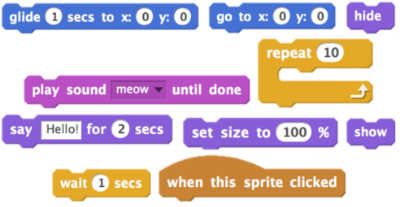
\includegraphics[scale=0.8]{10_ScratchBloks.png}
	\caption{{10 Scratch Bloks}}
	\label{fig:10Bloks}
\end{figure}

Den eneste programmet kan lytte på, er om en sprite klikkes eller ej.

\subsection{Version 0.1:}

Hypotese:

\begin{figure}[ht]
	\centering
	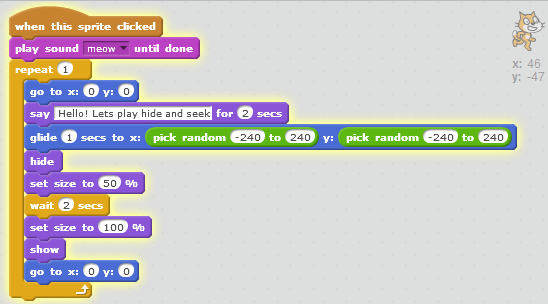
\includegraphics[scale=0.8]{10_ScratchBloks_Version01.png}
	\caption{{10 Scratch Bloks}}
	\label{fig:Version_0.1}
\end{figure}

\begin{itemize}
	\item Når vi klikker på vores sprite vil den begynde at miave.
	\item Gå til sin startposition og sige Let’s play hide and seek.
	\item Bevæge sig til et tilfældigt x,y koordinat mellem minus 240 og 240.	
	\item Så skjules spriten og den halveres i størrelse.
	\item Scriptet venter i 2 sekunder.
	\item Genskaber original størrelse (Trinnet er inkluderet for at bruge størrelses-commands).
	\item Spriten dukker op på det koordinat hvor den gemte sig.
	\item Spriten går tilbage til startposition.
\end{itemize}

\subsection{Resultat:}

\begin{itemize}
	\item Når der klikkes \textbf{første gang} miaver katten.
	\item Følgende gentages \textbf{en gang}.
	\begin{itemize}
		\item Går til sin startposition og udtaler sin besked
		\item Bevæger sig til et tilfældigt x,y koordinat mellem minus 240 og 240 i løbet af 1 sekund
		\item Herfra skjules spriten og vi kan først observere igen når den dukker op igen og vender tilbage til sin startposition
	\end{itemize}
\end{itemize}

\textit{Scriptet opførte sige i nogen grad som forventet, dog:}

Når man ændrer størrelsen med 50% er da af spritens originalstørrelse og ikke nuværende størrelse

Når spriten er hidden kan man ikke trykke på den
Det viser sig at fladen ikke er kvadratisk og desuden kan spriten flytte sig uden for baggrunden, altså må man tage højde når man programmerer x- og y-koordinater.

\subsection{Version 1.0:}

\begin{figure}[ht]
	\centering
	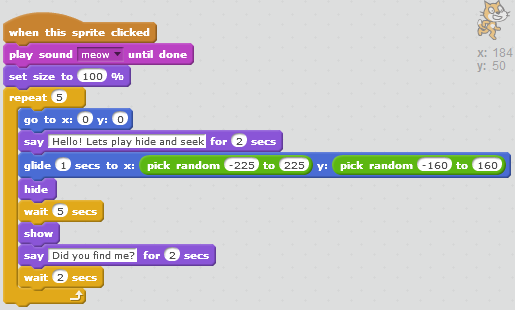
\includegraphics[scale=0.8]{10_ScratchBloks_Version1.png}
	\caption{{10 Scratch Bloks}}
	\label{fig:Version_1.0}
\end{figure}

Changelog:    

\begin{itemize}
	\item Starter med at etablere spritens originalstørrelse.
	\item Gentager sig selv \textbf{5 gange istedet}.
	\item Katten gemmer sig i længere tid.
	\item Katten slutter af med at sige “Did you find me?”
	\item X- og Y-koordinater er nu tilpasset bedre, bl.a. er fladen ikke kvadratisk så Y-aksen skulle tilpasses yderligere.
	\item Fjernede X- og Y-koordinat nulstillingen i slutningen af repeat loopet, da X- og Y-koordinat nulstillingen sker i det første trin der udføres i loopet. 
\end{itemize}


Vi har dog brugt en grøn ‘Vælg tilfældig’-boks\\

Link til programmet: \\
\url{https://scratch.mit.edu/projects/120575598/}





%----------------------------------------------------------------------------------------

%----------------------------------------------------------------------------------------
%	PROBLEM 3
%----------------------------------------------------------------------------------------

\section{1.2}

\textit{Hvilket slags spil vil vi lave?}\\

Vi sigtede i gruppen efter at lave et simpelt spil, hvor fokus kunne ligge på programmeringen i scratch i stedet for at bruge en masse tid på gamedesign.\\

Simpel hop over forhindringer i 2d sidecrolling miljø!

\subsection{Spilkoncept}

Katten skal undgå at blive bidt af hunden ved at hoppe over hunden. Hver gang man hopper over hunden får man et point, der tælles oppe i venstre hjørne. Hundens hastighed øges ydermere for hver point man scorer. Dette skaber en dynamisk sværhedsgrad der tilpasser spillerens evne.\\

\begin{figure}[ht]
	\centering
	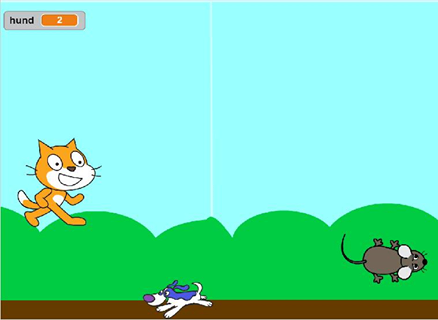
\includegraphics[scale=0.5]{Scratch_Game.png}
	\caption{{Scratch Spil}}
	\label{fig:screen_dump}
\end{figure}

\clearpage
\subsection{Programmering}

Som den mest fundamentale funktion i spillet skal katten kunne hoppe over hunden.\\

\begin{figure}[ht]
	\centering
	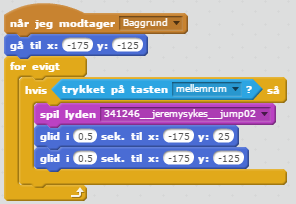
\includegraphics[scale=1]{jump.png}
	\caption{{Hoppe mekanismen for katten}}
	\label{fig:jumpCat}
\end{figure}

Når katten modtager startmeddelelsen (Baggrund), vil den altid antage sin startposition givet ved koordinaterne (x:-175, y:-125). Derefter vil den for evigt vente på spilleren giver kommandoen mellemrum, hvor efter den i et bestemt tidsinterval vil rykke hundred enheder op på y og ned.\\

Dernæst skal vores kat holde øje med om den støder ind i hunden.\\

\begin{figure}[ht]
	\centering
	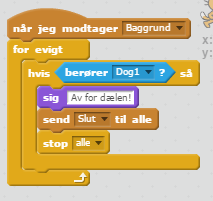
\includegraphics[scale=1]{collision.png}
	\caption{{Kollision med hunden}}
	\label{fig:coll}
\end{figure}

Når spriten modtager vores startmeddelelse holder katten for evigt øje med om den berør en hund. Hvis katten på et vilkårligt tidspunkt berør hunden siger den 'Av for dælen!' og vil dernæst sende en besked rundt som får Game over-spriten til at dukke op, inden den stopper alle andre scripts.\\
\clearpage
Vores spil er også afhængigt af at der skabes hunde som katten undgå\\

\begin{figure}[ht]
	\centering
	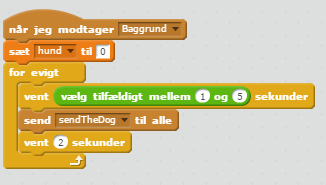
\includegraphics[scale=1]{baggrunddog.png}
	\caption{{Sender signal ved tilfældige intervaller til at skabe og sende hunde}}
	\label{fig:dog_sig}
\end{figure}

Når startmeddelelsen sendes rundt, nulstilles vores hundevariabel for det første, idet den angiver hvor mange hunde man har undgået. Derefter vil hundene resten af spillet skabes i et interval på 1-5 + 2 sekunder, de to sekunder er lagt til for at sikre en hvis reaktionstid for spilleren. Når en hund skal skabes sendes beskeden 'sendTheDog'. (Vi kunne dog have ændret det tilfældige valg til 3-7 sekunder og opnå samme resultat som ved at fjerne en vent 2 sekunder block)\\

\begin{figure}[ht]
	\centering
	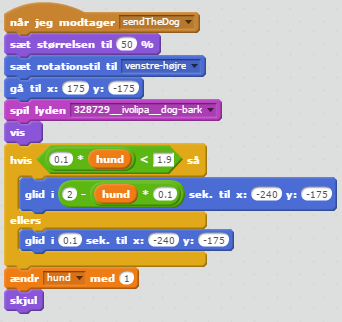
\includegraphics[scale=1]{sendthedog.png}
	\caption{{Initialisere hunden og bestemmer hastigheden på baggrund af point}}
	\label{fig:dog_init}
\end{figure}

Metoden for glideanimationen af hunden fra højre til venstre starter når signalet 'sendTheDog' bliver modtaget. Først bliver hundens størrelse, retning og startposition angivet for så at afspille en "wow" lyd og vise hunden. Dernæst skal hunden glide 0.1 sekunder hurtigere for hver hund man hopper over. Der er sat en begrænsning hvor hunden minimalt vil glide gennem banen med 0.1 sekunder. 


%----------------------------------------------------------------------------------------
%----------------------------------------------------------------------------------------
%	PROBLEM x
%----------------------------------------------------------------------------------------



%----------------------------------------------------------------------------------------

\end{document}